%% REVISE FOR KEYWORD-ABBREVIATION REFERENCES and ABBREVIATION DETAILS
%%% CHAPTER Introduction ------------------------------begin----
%Quotes to have

\chapter{Introduction}
\section{Motivation}
Developing and distributing effective software is one of the most important concerns of today's software-driven fields. Effective software is surely needed in almost every part of embedded systems, especially in the fields of automotive, robotics, defense, transportation, electrical instruments, autonomous and cyber-physical systems. Quality software involvement in fields such as the ones that are mentioned created a great demand for parallel software development in the last ten years. This great demand caused software engineers in especially IT and embedded system sector to study parallel computing along with multi- and many- core systems.

The digitalization of almost every aspect of our lives as we know it requires systems to be more and more complex each passing day. While some years ago the computers had single-core processors, today almost every single computer has at least a couple of cores in their processors. The advancements in processors allowed development of more advanced systems with efficient software. The super computers currently NASA (The National Aeronautics and Space Administration) uses for collecting information are said to record as much data as it has been collected in the entire the world history in just four years. This example should show that how complex applications can be in the century we are living in. Furthermore, one of the most trending topics Cloud Computing, which is being studied to make use of complex computing power of super computers' remotely to public users, is being researched and it will benefit greatly from the advancements in the field of parallel computing.

While parallel computing is used for achieving more complex software, it is also widely used in more basic and cheap processors in order to achieve more tasks with less resource consumption and cost. This is achieved by proper scheduling techniques. Furthermore, with an efficient software distributed efficiently to a processor's cores, one could also make use of less energy consumption features by applying techniques such as under-clocking a processor. To summarize, developing efficient parallel software is not only useful in achieving advanced computing capability but also can help to achieve less energy and resource consumption, thus decreasing the cost of systems and making them more environment-friendly.

\section{Objective}
Even though achieving concurrency using parallel computing is crucial, it might lead to error-prone systems if software is not planned and executed properly. Developers have to consider using the right software and also have to determine and plan not only the hardware constraints but also the software constraints in order to create an efficient and reliable software.

Before its execution, parallel software have to be delicately planned. The first stage of the parallel software development, planning stage, involves several activities such as Modeling, Partitioning, Task generation and Mapping. In the modeling stage, hardware and software model needs to be created. While software model is described by defining runnables, labels, label accesses, runnable activations and software constraints; the hardware model is described by defining processor details, hardware system clock and core information. After the modeling activity, partitioning is done that determines which group of runnables belong together. Partitioning results are combined with system constraints in order to generate tasks. Final activity, Mapping, involves laying out the details about pinning generated tasks to available hardware units and their cores.

While there are some commercial tools that provide easement in the parallel software development, recent study done in Germany, namely AMALTHEA4public \cite{ICPDSSE} \cite{amalthea4publicweb}, aims to provide planning and tracing tools especially for multi-core developments in automotive domain with several open source development tools. The branch of AMALTHEA4public, APP4MC project \cite{app4mcproposaleclipse} provides an Eclipse-based tool chain environment and de-facto standard to integrate tools for all major design steps in the multi- and many-core development phase. A basic set of tools are available to demonstrate all the steps needed in the development process. The APP4MC project aims at providing \cite{app4mcproposaleclipse}:

\begin{itemize}
	\item A basis for the integration of various tools into a consistent and comprehensive tool chain.
	\item Extensive models for timing behaviour, software, hardware, and constraints descriptions (used for simulation / analysis and for exchange).
	\item Editors and domain specific languages for the models.
	\item Tools for scheduling, partitioning, and optimizing of multi- and many-core architectures \cite{app4mcproposaleclipse}.
\end{itemize}

The author aims to investigate and evaluate APP4MC's performance with real-world distributed multi-core system in several aspects such as core utilization, energy consumption and resource usage while studying efficient parallel computing and tracing activities at his time with Project AMALTHEA4public.

\section{Methodology}

Automotive or any vehicle control related field tends to require very complex systems. In a real-life automotive application, amount of hardware nodes and software nodes are high in number. Since the main focus of the APP4MC environment is to provide parallel computation tools for automotive domain, a demonstrator is required that is closely related to automotive domain and that can be used for troubleshooting APP4MC. For that purpose, a demonstrator RC-Car called A4MCAR is developed. Although an RC-Car does not match up the number of nodes used in real vehicles, the A4MCAR has several nodes and a distributed architecture, thus matching a vehicle's distributed architecture such as the AUTOSAR used in vehicles. Furthermore, A4MCAR can be used for automotive-like applications that involve motor driving, navigation, sensor driving, and autonomous features.

The demonstrator, A4MCAR, is equipped with a distributed architecture that involves a 16-core multi-core microcontroller development board (XMOS xCore-200 eXplorerKIT) and a 4-core single board computer (Raspberry Pi 3) with Linux OS. The software nodes with respect to their priorities and low-level and high-level purposes are distributed along those hardware modules. The demonstrator is not only designed to match up the capabilities of a real vehicle but also involves parts that are related to semi-autonomous driving and control. It can handle wifi and bluetooth connection requests and drive itself accordingly over a web interface or an Android application. Since A4MCAR is specifically designed as a demonstrator, it has the capability to monitor and visualize core utilization and display it using a touchscreen or its web interface. Furthermore, it is equipped with four ultrasonic sensors and a camera with image processing embedded to support its autonomous driving and web interface streaming functions.

In this paper, the development and parallelism evaluation of the demonstrator A4MCAR as well as the studies on parallel computing and tracing options are discussed. Obtained results are used in APP4MC for better development. The remainder of this paper is organized as follows: Section 2 is dedicated to Multi-core programming while Section 3 is dedicated to explaining APP4MC environment. In Section 4, the demonstrator design and implementation will be explained. After Section 4, Section 5 and 6 will involve Information Tracing and System Modeling with APP4MC and Effective Parallelism Evaluation, respectively. The paper will be concluded with Section 7.

%%% CHAPTER Introduction ------------------------------end----
%%% CHAPTER Multi-core Programming ------------------begin----
\chapter{Multi-core Programming}  %Chapter outline is work in progess..
\section{Distributed and Parallel Systems} %and Distributed systems
\subsection{Introduction} %Definitions and intro
\subsection{Memory Architectures} %characteristics + architectures
\subsubsection{Computers with Shared Memory Organization}
\subsubsection{Computers with Distributed Memory Organization}
\subsubsection{Computers with Distributed and Shared Memory Organization}
\subsection{Memory Communication} %Distributed + shared mem comm techniques
\section{Introduction to Parallelism} 
\subsection{Levels of Parallelism}
\subsection{Characteristics, Challenges and Constraints of Parallel Systems} % involves co-design stages (parallelization of programs pp.108) partitioning mapping egc. + Also advantages and disadvantages

\subsection{Coordination and Mutual Exclusion}
\subsubsection{Parallelism Terminology}  %terminology: intro, process, task ,thread, runnable etc
\subsubsection{Problems in Coordination} % race cond, deadlock, livelocketc. 
\subsubsection{Mutual Exclusion} %mutex semaphore etc.
\subsection{Optimization of Parallelization}
\section{Multi-core Processor Architecture}
\section{Scheduling} %and schedulers
\section{Real-time Parallelization Trends in Practice: RTOS, MPI, OpenMP, Pthreads, Java Threads} %x Give example of FreeRTOS for RTOS.
\section{Importance of Multi-core computing to automotive industry: AUTOSAR}

%%% CHAPTER Multi-core Programming ------------------end----
%%% CHAPTER APP4MC Development Environment ----------begin----
\chapter{APP4MC Development Environment}
\section{Introduction} %Motivation
\section{Features}
\section{Modeling}
%%% CHAPTER APP4MC Development Environment ------------end----
%%% CHAPTER A4MCAR ----------------------------------begin----
\chapter{Distributed Multi-core Demonstrator (A4MCAR) Design and Implementation}
\section{System Overview}
As introduced in the Introduction chapter, A4MCAR is a demonstrator RC-Car for the APP4MC development environment. A4MCAR provides a distributed multi-core architecture that allows the demonstration of embedded low-level and high-level applications. 
\subsection{System Features}
\begin{figure}[htb]
	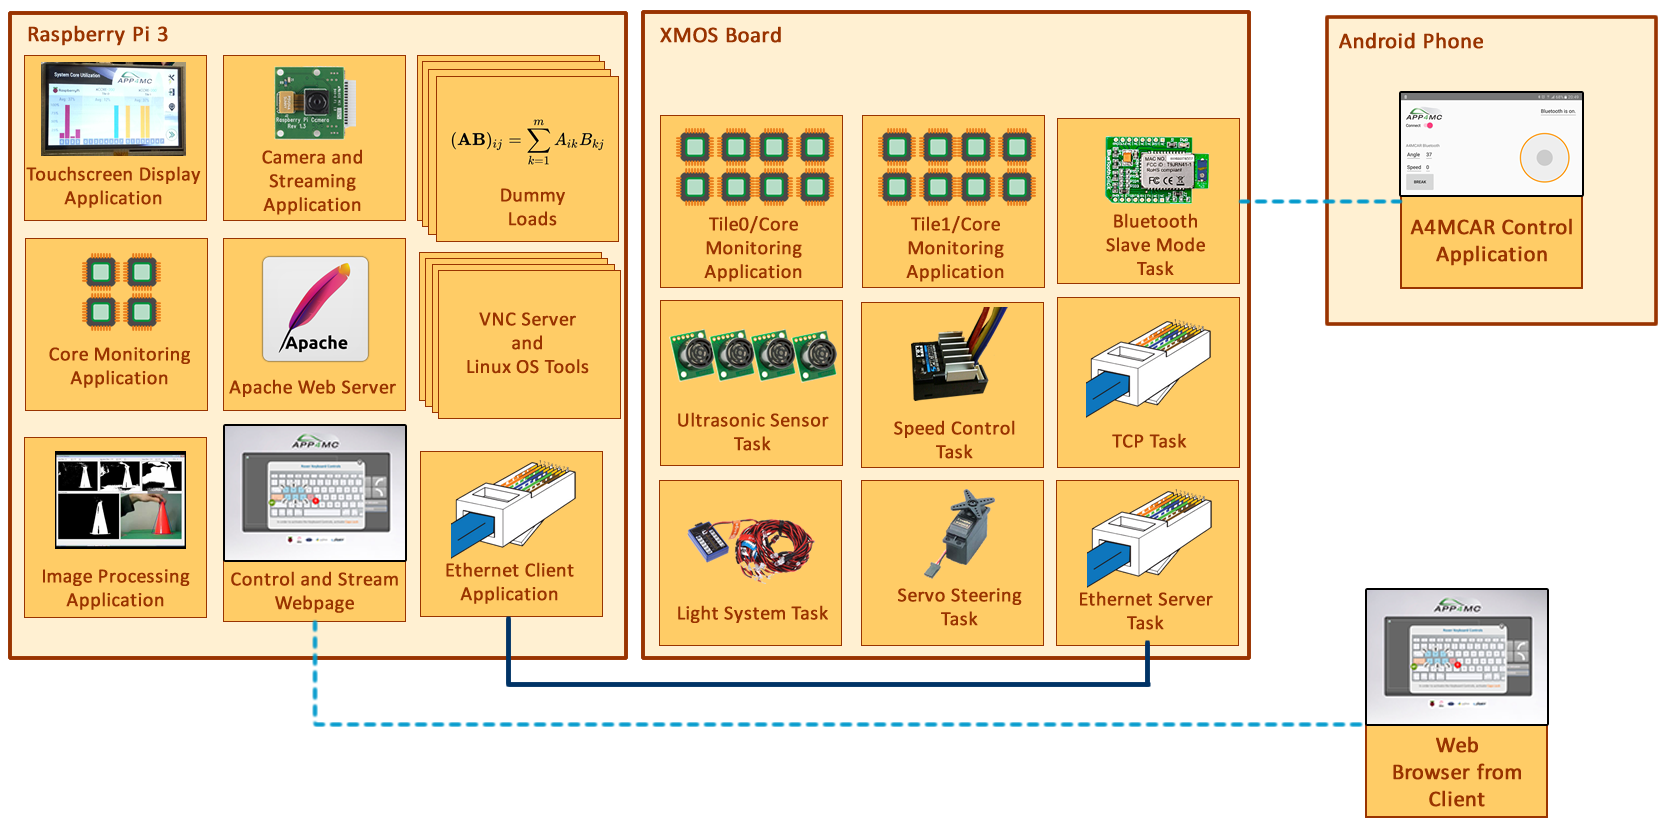
\includegraphics[scale=0.3]{content/images/tasksoverall.png}
	\caption{Applications developed and/or maintained for A4MCAR}
	\label{fig:tasksoverall}
\end{figure}
\subsection{Infrastructure}
\subsubsection{XMOS XS-1 Infrastructure}
\subsubsection{Raspberry Pi 3 Infrastructure}
\subsection{Sensors}
\subsection{Hardware Design and Interfaces}
\begin{figure}[htb]
	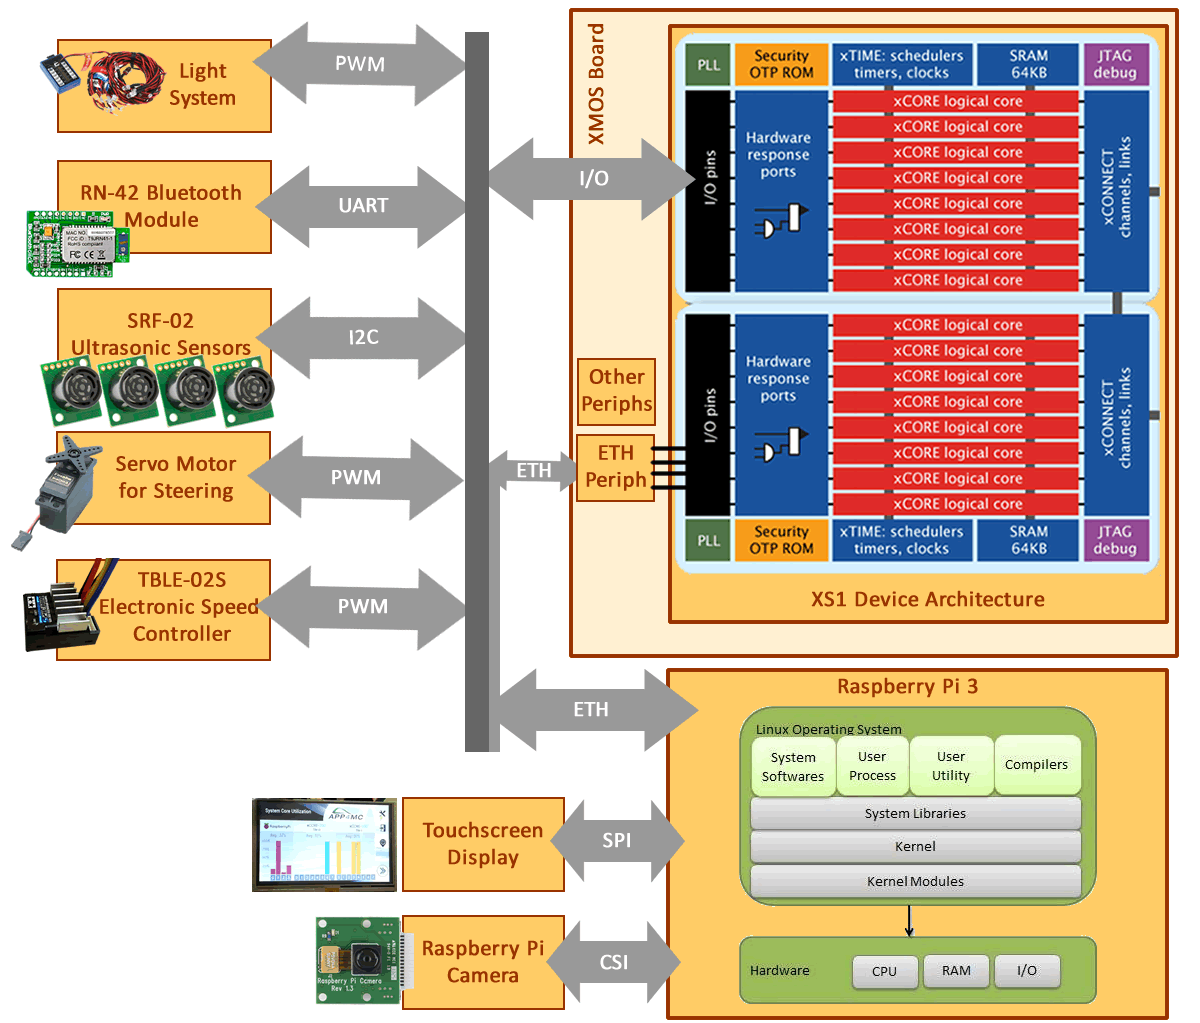
\includegraphics[scale=0.35]{content/images/hwoverview.png}
	\caption{Hardware overview of A4MCAR}
	\label{fig:hwoverview}
\end{figure}
\subsection{Safety and Power}
\subsection{Mechanical Design}
\begin{figure}[htb]
	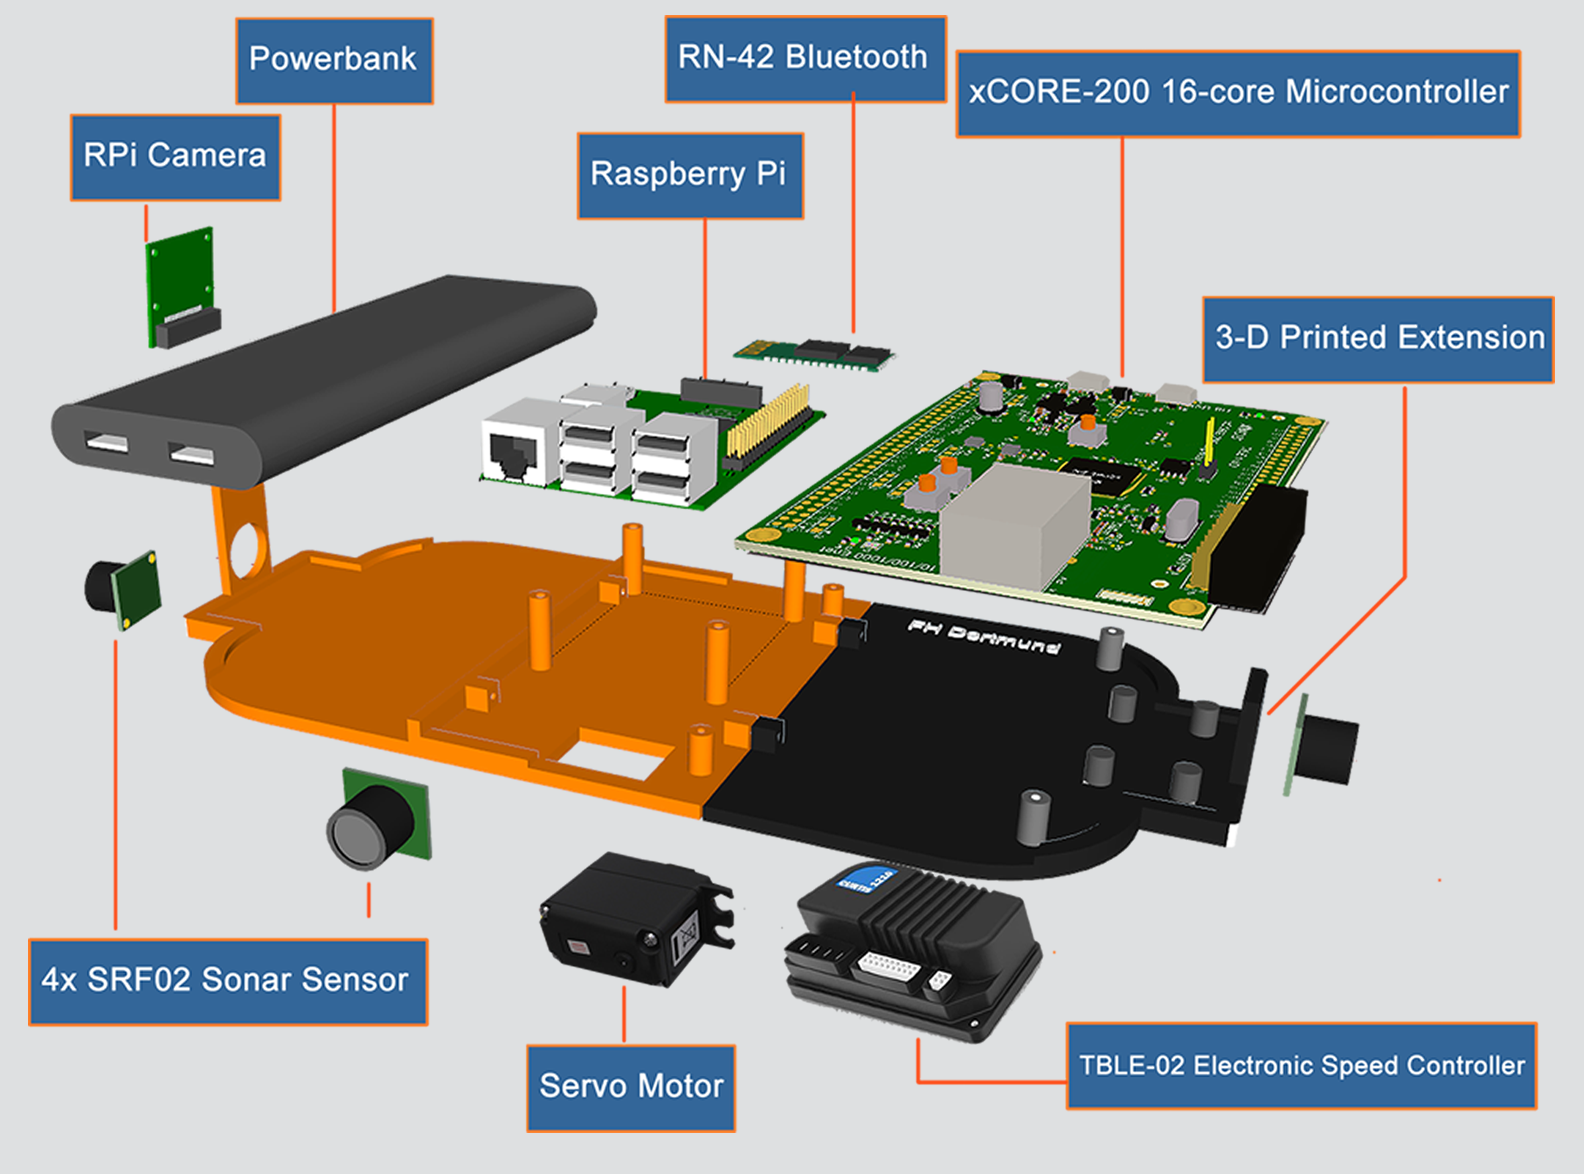
\includegraphics[scale=0.25]{content/images/mechanicaloverview.png}
	\caption{Mechanical overview of the A4MCAR}
	\label{fig:sysmlxmostasks}
\end{figure}
\section{Low-Level Module Design and Implementation}
\subsection{Overview}
\begin{figure}[htb]
	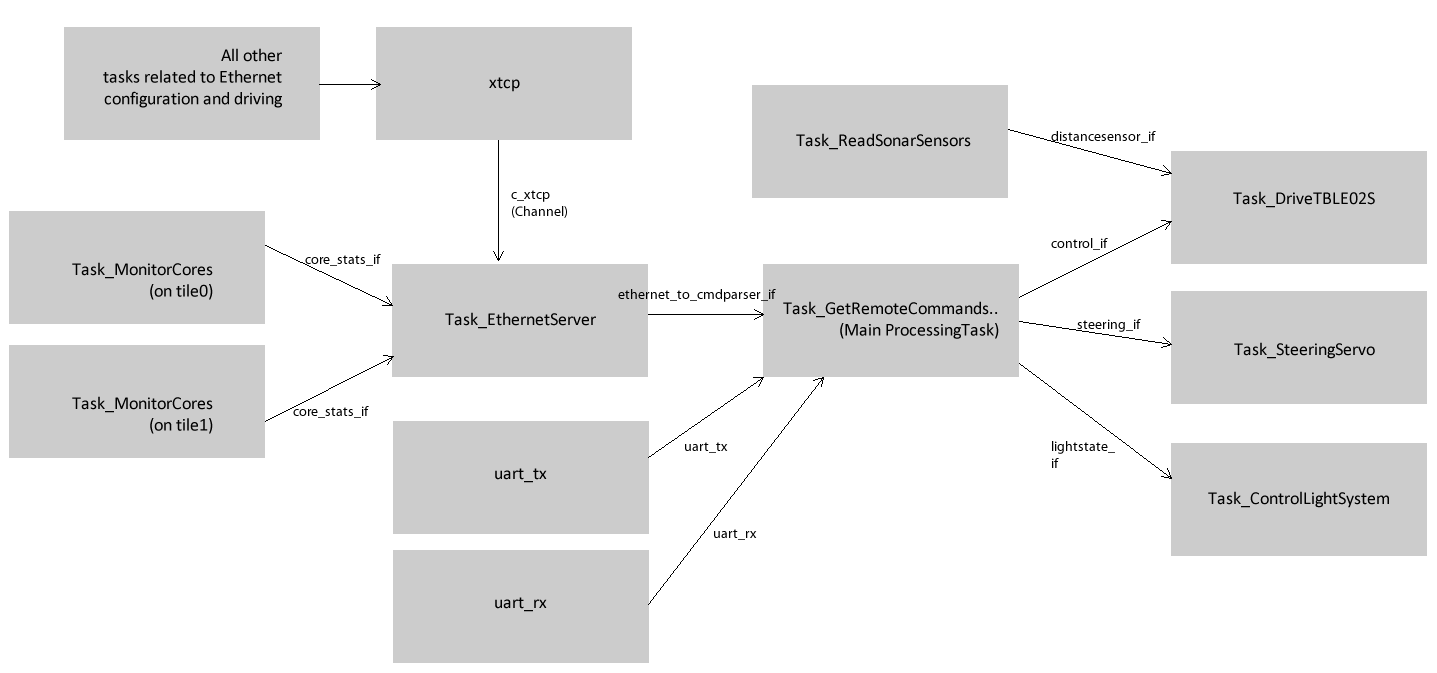
\includegraphics[scale=0.32]{content/images/sysmlxmostasksbrief.png}
	\caption{Brief block diagram for the developed tasks and interfaces}
	\label{fig:sysmlxmostasks}
\end{figure}
\begin{figure}[htb]
	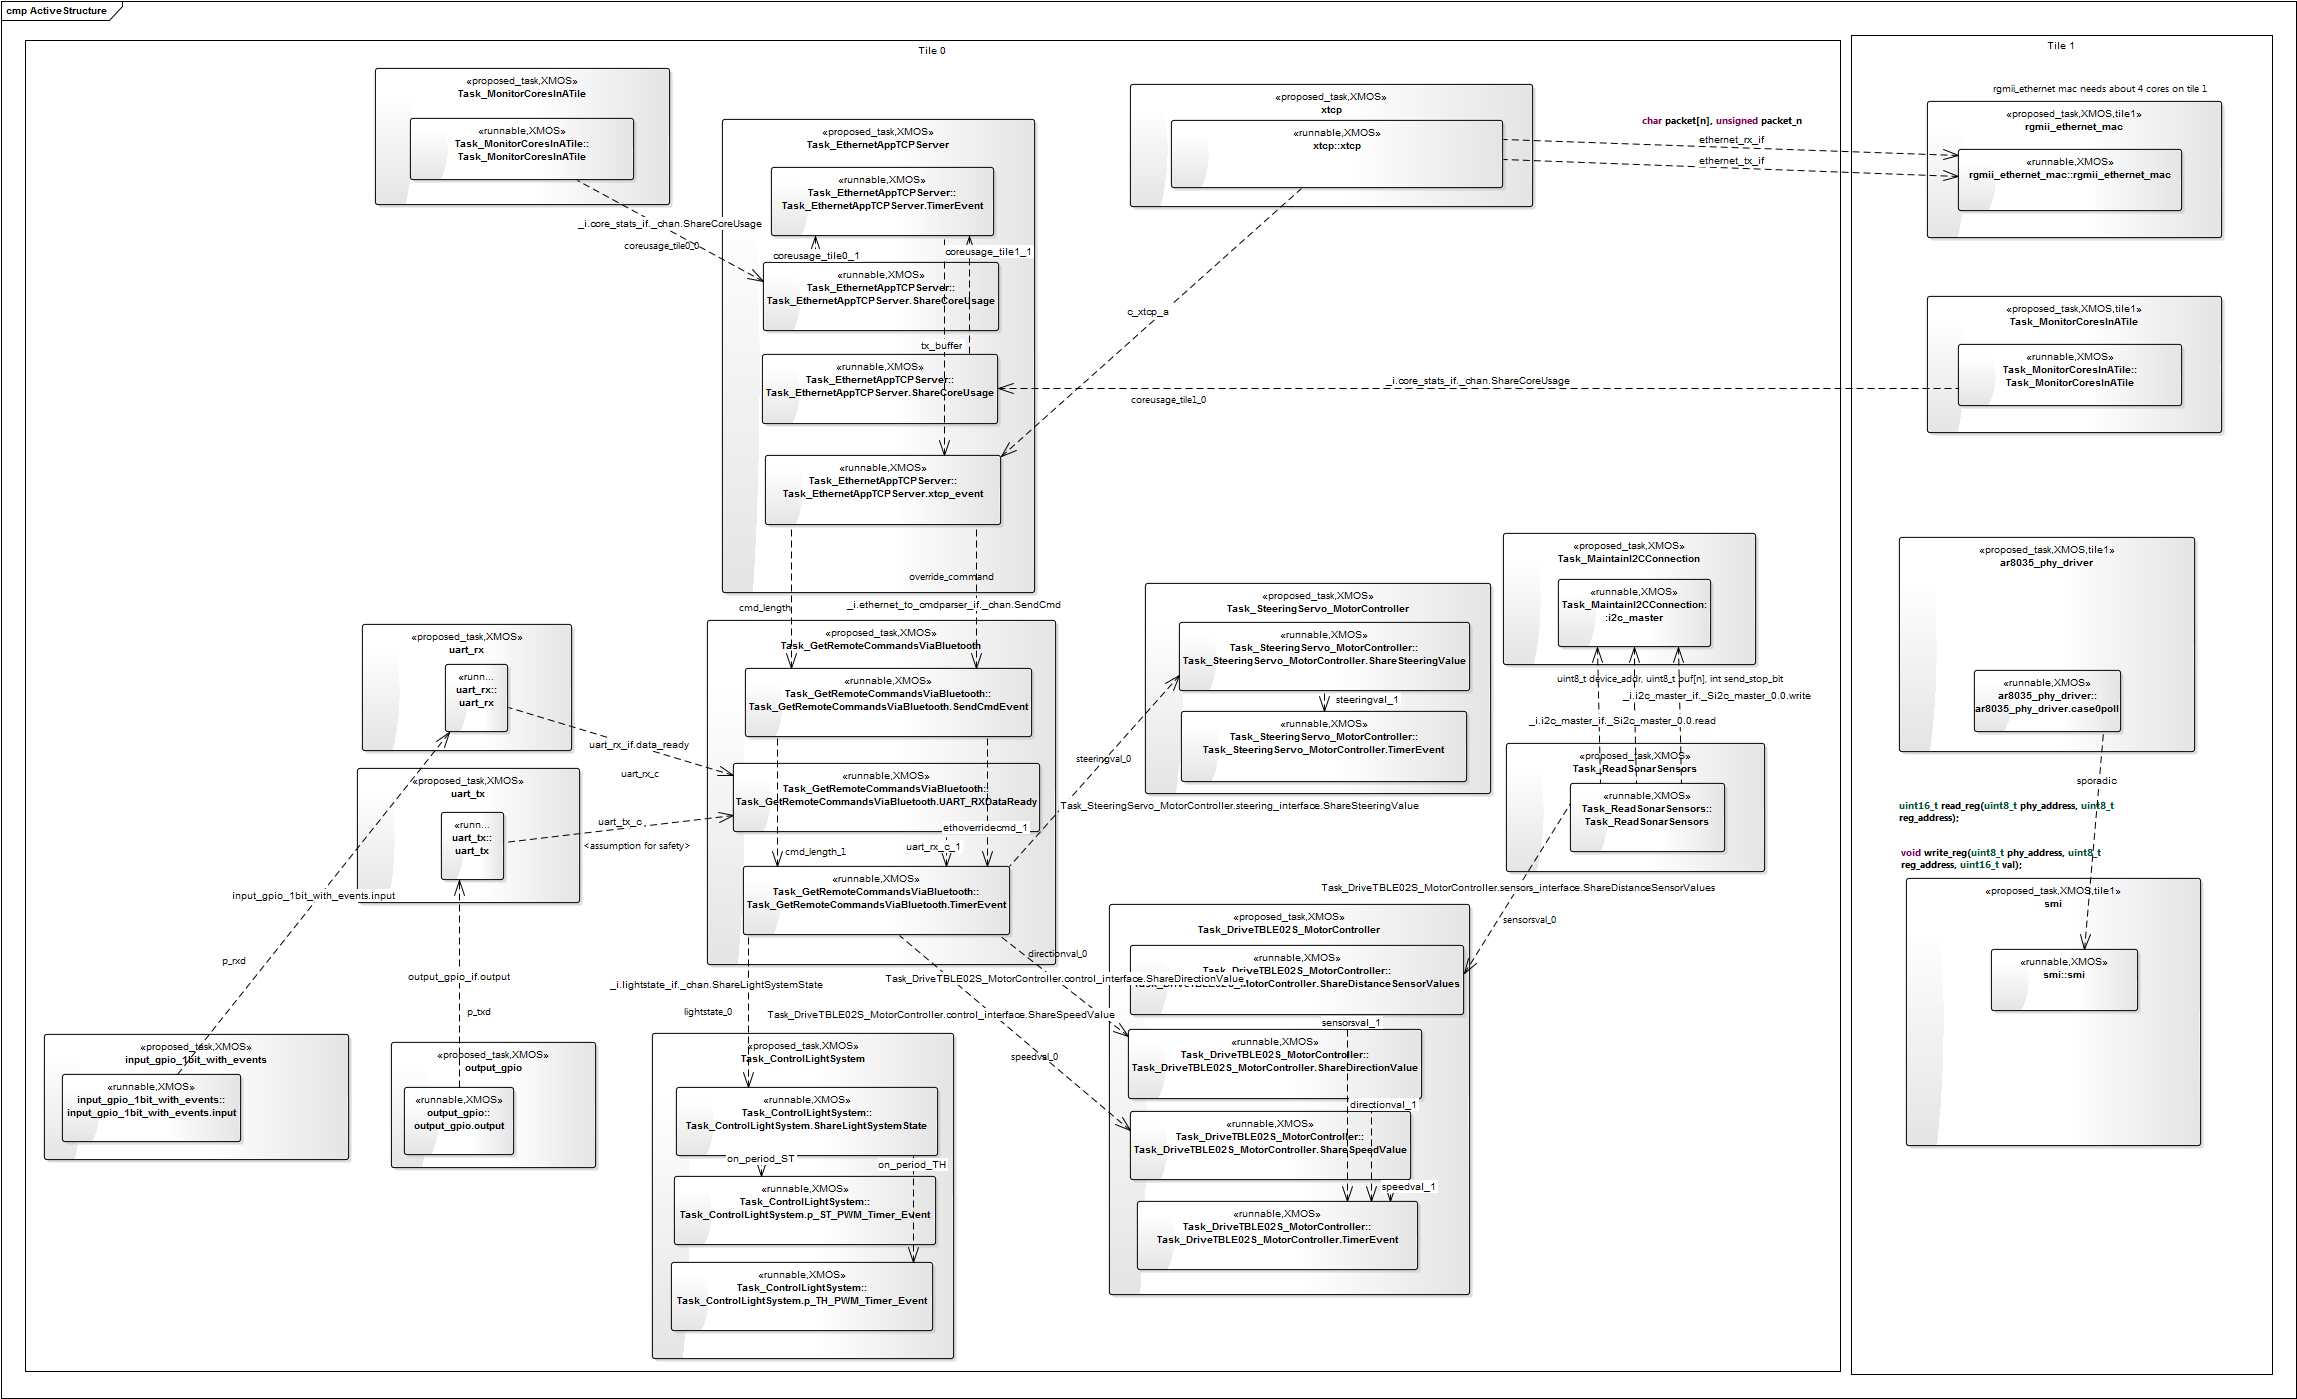
\includegraphics[scale=0.21]{content/images/sysmlxmostasks.png}
	\caption{Block diagram for the developed tasks and interfaces}
	\label{fig:sysmlxmostasks}
\end{figure}
\subsection{Actuation}
\subsubsection{Acceleration}
\subsubsection{Steering}
\subsection{Proximity Sensing}
\subsection{Lighting System}
\subsection{Bluetooth Communication}
\subsection{Ethernet (TCP) Communication}
\subsection{Core and Tile Monitoring}
\section{High-Level Module Design and Implementation}
\subsection{Overview}
\subsection{Core Monitoring}
\subsection{Web Server and its Applications}
\subsubsection{Web Server}
\subsubsection{Web Page Design and Implementation}  %Very briefly but include technologies and how it works, jquery-ajax, html,css and so on.
\subsubsection{Controlling A4MCAR via Web Page}
\subsubsection{Camera Streaming}
\subsubsection{Core Utilization Display}
\subsection{Dummy Loads}
\subsection{Image Processing with OpenCV}
\subsection{Touchscreen Display}
\subsubsection{Touchscreen Display Implementation}
\subsubsection{Touchscreen Display Functions}
%Linux tools and created .sh scripts will be in Section (5)
\subsection{VNC Server}
\subsection{Additional Bash Scripts}
\section{Android Application Implementation}
%%% CHAPTER A4MCAR ------------------------------------end----
%%% CHAPTER Information Tracing and System Modeling --------begin----
\chapter{Information Tracing and System Management}
\section{Low-Level Module Information Tracing and System Management}
\subsection{What kind of information needed?}
\subsection{Information Tracing via xTimeScheduler}
\subsection{Information Tracing via APP4MC}
\subsection{Distribution of Tasks to Cores}
\subsection{Discovering Energy Consumption Features}
\section{High-Level Module Information Tracing and System Management}
\subsection{What kind of information needed?}
\subsection{Information Tracing via Linux Kernel}
\subsubsection{Linux Kernel Basics} %processes,threads, scheduling
\subsubsection{top} %including threads
\subsubsection{Process Management using ps Command} % getting pid, getting killing processes
\subsubsection{Using perf to get number of instructions}
\subsubsection{dis}
\subsubsection{objdump}
\subsubsection{Using perf to get scheduling information}
\subsubsection{kernelshark}
\subsubsection{lttng and TraceCompass}
\subsubsection{proc folder}
\subsubsection{psutil}
\subsection{Distribution of Processes using taskset in Linux}
\subsection{Discovering Energy Consumption Features in Linux with cpufrequtils}


%%% CHAPTER Information Tracing and System Modeling --------end----
%%% CHAPTER Effective Parallelism Evaluation --------begin----
\chapter{Effective Parallelism Evaluation}
\section{Low-Level Module Parallelism} %in RCCAR
\subsection{System Model}
\subsection{Efficiency Model}
\subsection{Evaluation of Different Distributions}
\subsection{Results from APP4MC Distribution}
\section{High-Level Module Parallelism}
\subsection{System Model}
\subsection{Efficiency Model}
\subsection{Evaluation of Different Distributions}
\subsection{Results from APP4MC Distribution}
%Distributed system and embedded systems characteristics.... scalability etc.. real-time system.
%Also description of our systems characteristics.

%x APPSTACLE emphasis
%Quote:
%The main benefit for having release, start, (preemption), end, and deadline values is deriving efficiency. For each task instance, you can calculate e.g. the slack time, that indicates how much time is left before its next execution. The higher the slack time is, the better was its execution. Different scenarios and different tasks have different profiling results (slack time is just one of them) and their investigation leads to a precise assessment of software distribution!
%(Maybe also involve deadline misses..)

%the period usually is the deadline. as soon as execution time exceeds this, you must indicate a “deadline miss” it can lead to system failure or even cause (in the automotive domain) person harm. Think of a break application that must react within e.g. 1ms to ensure accurate braking.
%To answer your question: it is ok, but you must indicate the deadline miss
%you should ‘design’ (since you do not have any timing requirements) the periods in a way that they should meet deadlines
%f you want to show that unser a certain period definition, deadline misses definitely occure (e.g. sequential execution) than you can, for sure, design the periods in that way
% you can measure different scenarios (periods) though (i recommend that)

%Design of rpi apps and timing for real-time scheduling...
%Formulas and how the display timing designed.
%How deadlines designed with periods conforming to parallel distribution

%Linux OS overheads + App Timing additions overhead..


%Give scheduling image.. and explain..

%Real-time Scheduling in Linux?????
%time.time (real time) vs time.clock (processor time) (does not count cpu sleeps)

%Overall mean slack time -> longer means distribution is better.
% Core execution times should be same but Response times  (= GETs ) will slightly differ.
%Why dont we have IPT? which causes Response times = GETs

%Different measurements -> scenerios -> results evaluation using kernelshark, lttng AND TraceCompass!!! and other tools. (also include image processing app in some scenerios)

%Online efficiency calculation using rpi and offline distribution analysis.

% Real-time EMPHASIS REALLY IMPORTANT. MAKE A CHAPTER ON THAT

%Why real-time computing not supported in ARM architecture, especially Raspberry Pi ? (search this!!)

% Thread analizini de yapalim
%top -H -p <pid> or ps -T -p <pid>
%Clock speed > Power

%Problems measuring efficiency using slack time with Rpi:
%There needs to be a dynamic sleep time(period-exectime)
%time.timeshould be used instead of time.clock()

%x DVFS Dynamic Voltage and Frequency Scaling


%%% CHAPTER Effective Parallelism Evaluation --------end----
%%% CHAPTER Conclusion ----------------------------begin----
\chapter{Conclusion}

%%% CHAPTER Conclusion ------------------------------end----